\documentclass[a4paper]{book}
\usepackage{a4wide}
\usepackage{makeidx}
\usepackage{graphicx}
\usepackage{multicol}
\usepackage{float}
\usepackage{listings}
\usepackage{color}
\usepackage{textcomp}
\usepackage{alltt}
\usepackage{times}
\usepackage{ifpdf}
\ifpdf
\usepackage[pdftex,
            pagebackref=true,
            colorlinks=true,
            linkcolor=blue,
            unicode
           ]{hyperref}
\else
\usepackage[ps2pdf,
            pagebackref=true,
            colorlinks=true,
            linkcolor=blue,
            unicode
           ]{hyperref}
\usepackage{pspicture}
\fi
\usepackage[utf8]{inputenc}
\usepackage{doxygen}
\lstset{language=C++,inputencoding=utf8,basicstyle=\footnotesize,breaklines=true,breakatwhitespace=true,tabsize=4,numbers=left }
\usepackage{longtable,amssymb,amsmath,mathrsfs,fancyhdr,pdfpages}
\makeindex
\setcounter{tocdepth}{3}
\renewcommand{\footrulewidth}{0.4pt}
\newcommand{\smfrac}[2]{#1/#2}
\newcommand{\derr}[2]{\frac{\partial #1}{\partial #2}}
\newcommand{\fav}[1]{\widetilde{#1}}
\newcommand{\xav}[1]{\left\langle{#1}\right\rangle}
\newcommand{\tav}[1]{\overline{#1}}
\newcommand{\source}[2]{\ensuremath{\mathcal{S}_{#1}^{\mathrm{#2}}}}
\newcommand{\force}[2]{\ensuremath{\mathcal{F}_{#1}^{\mathrm{#2}}}}
\newcommand{\mr}[1]{\ensuremath{\mathrm{#1}}}
\newcommand{\sgse}{e}
\newcommand{\rese}{E}
\newcommand{\iftwocol}[2]{\if\else #2\fi}
\newcommand{\CFL}{\mr{CFL}}

\setcounter{tocdepth}{1}

\begin{document}
\begin{titlepage}
\vspace*{7cm}
\begin{center}
{\Large Dutch Atmospheric Large Eddy Simulation}\\
\vspace*{1cm}
{\large User manual}\\
\vspace*{0.5cm}
{\small \today}\\
\end{center}
\end{titlepage}
\clearemptydoublepage
\pagenumbering{roman}
\tableofcontents
\clearemptydoublepage
\pagenumbering{arabic}
\hypersetup{pageanchor=true}
\chapter{General Introduction}
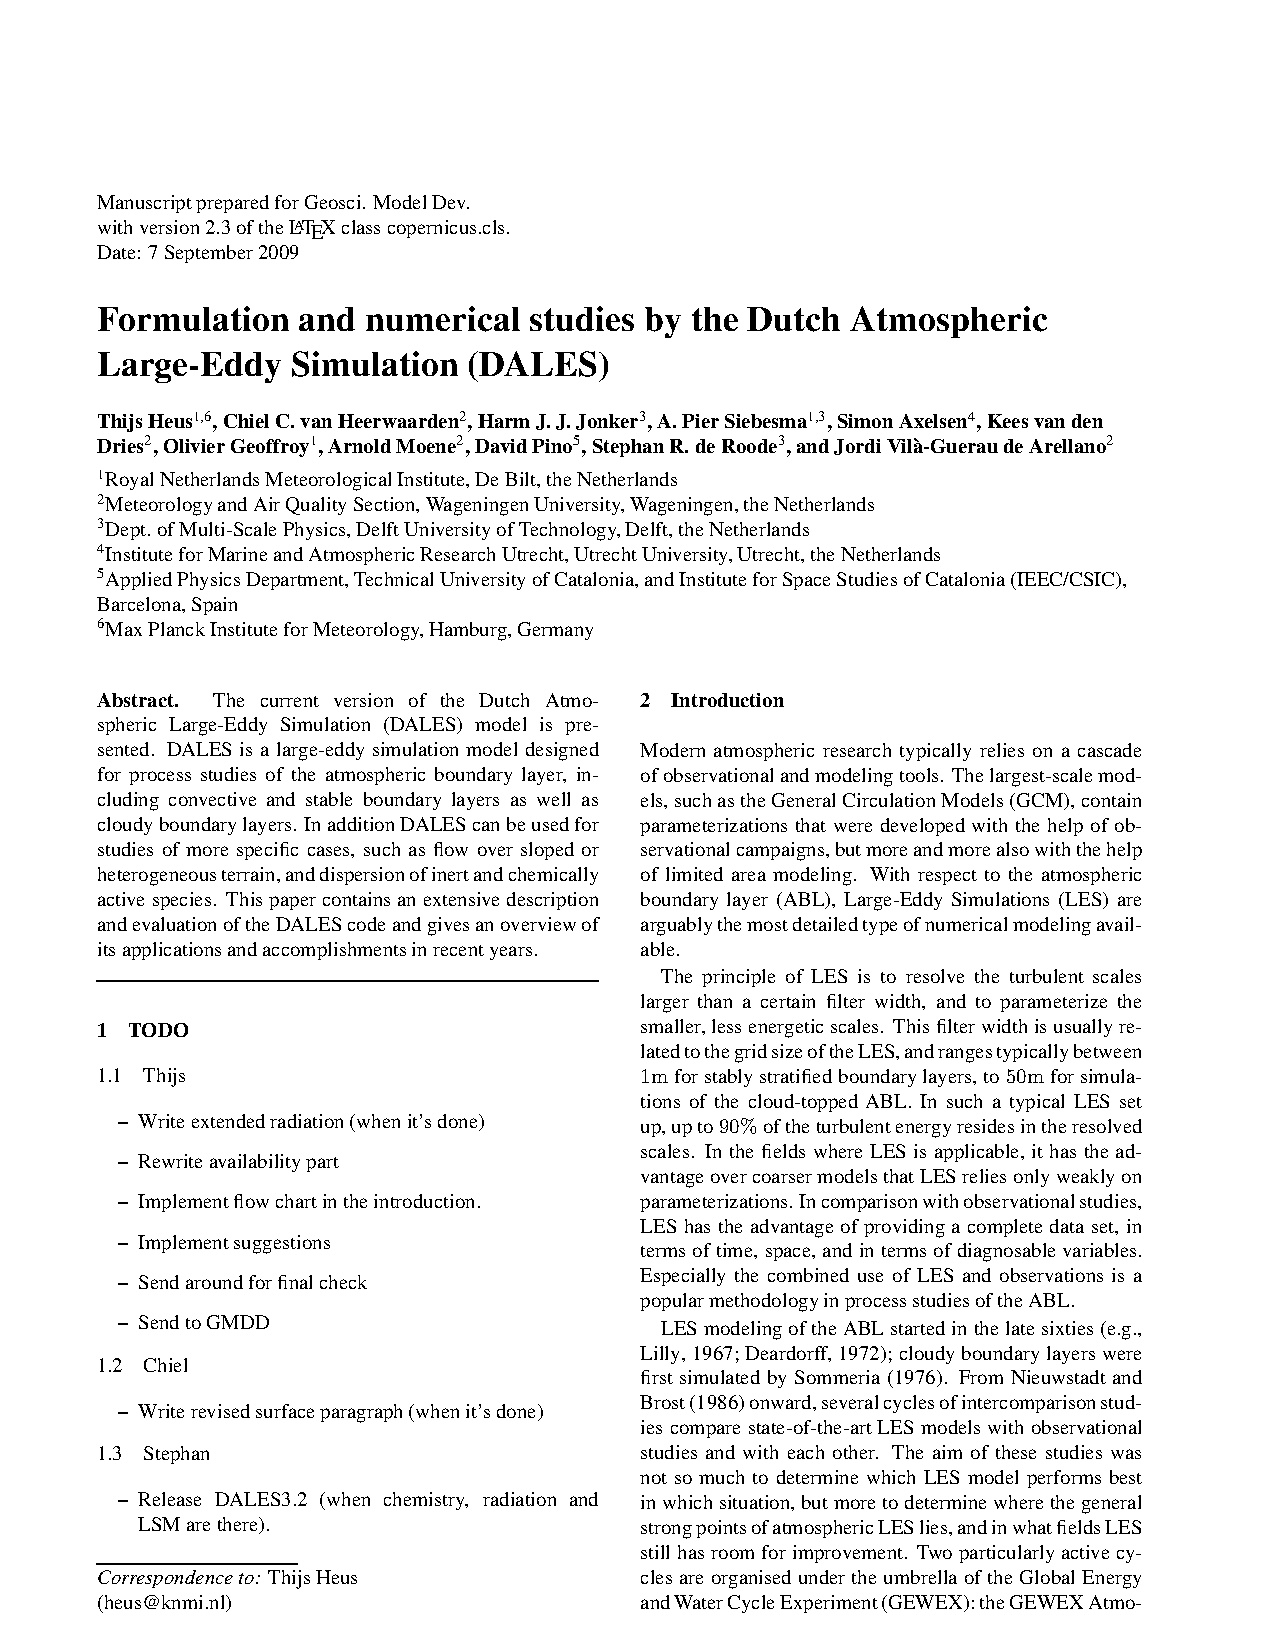
\includepdf[pages=-]{dales-article.pdf}
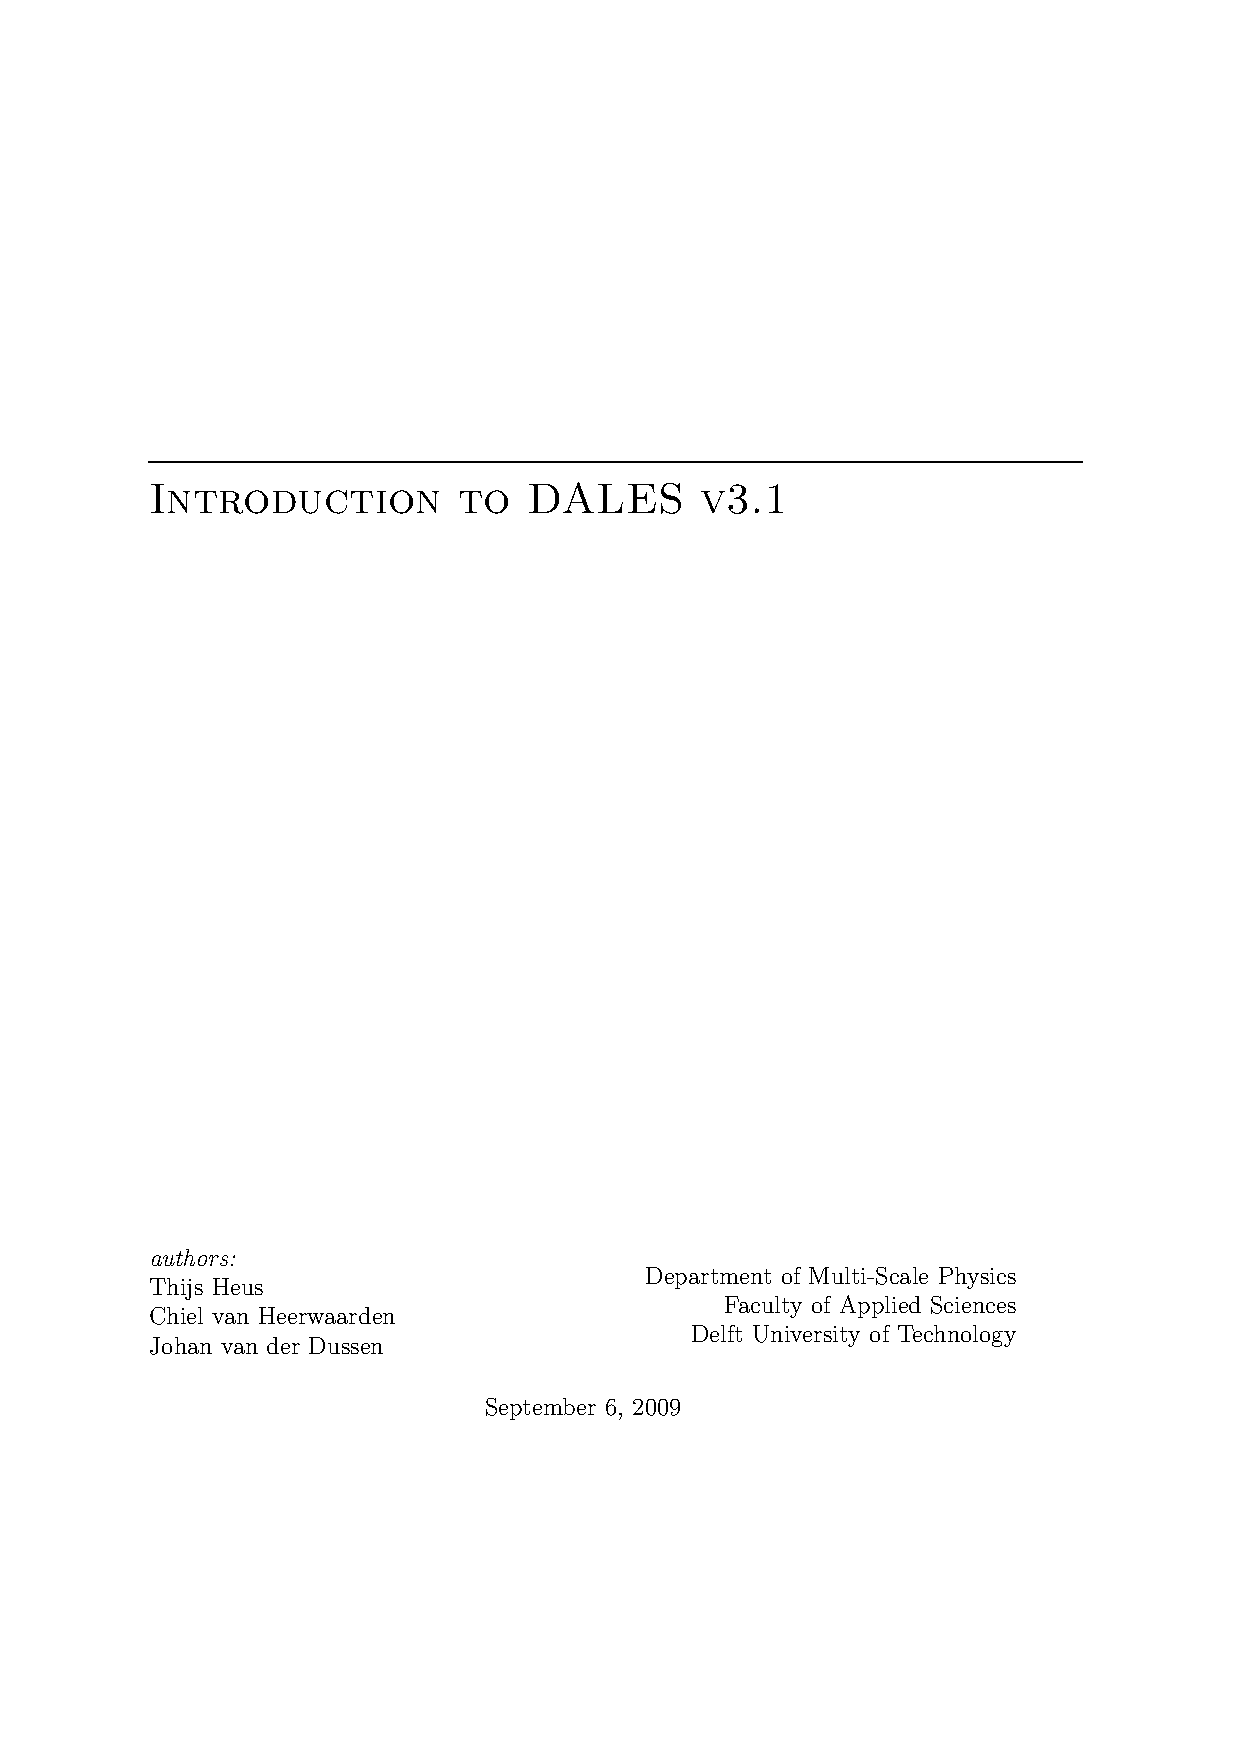
\includepdf[pages=-]{dales-manual.pdf}
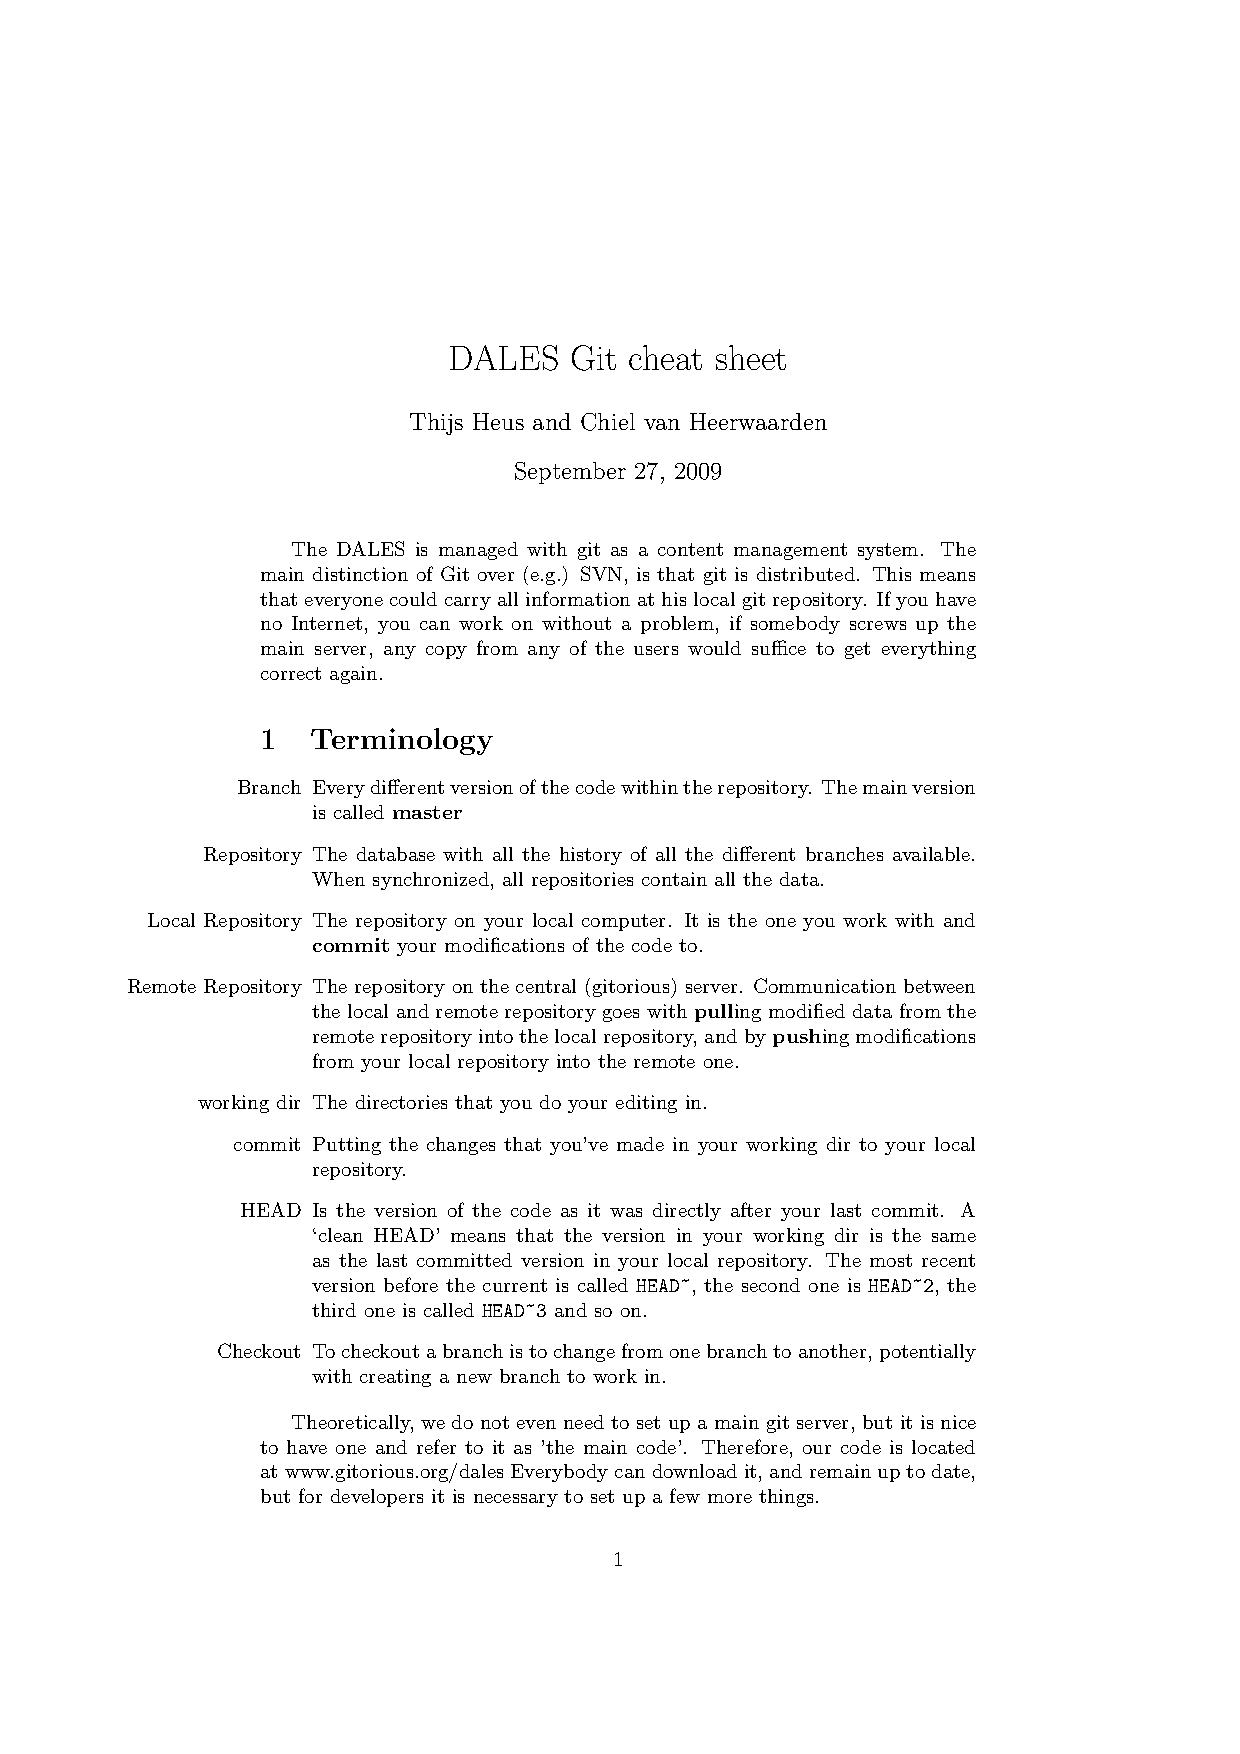
\includepdf[pages=-]{git_dales.pdf}